%%===============================================================
%%===============================================================
\chapter{OpenFCST \texttt{src} structure}
%%===============================================================
%%===============================================================

This chapter discusses the sections of the source folder in OpenFCST, i.e., the \texttt{src} folder.
%%===============================================================
\section{Directory tree}
%%===============================================================
OpenFCST contains six subfolders, namely:
\begin{itemize}
 \item \texttt{fcst} is the most important folder in OpenFCST \texttt{src}. It contains the include (*.h) and implementation (*.cc) files for OpenFCST. Inside this folder the following sub-folders can be found:
 \begin{itemize}
  \item \texttt{include} contains all include files (*.h)
  \item \texttt{source} contains all source files (*.cc)
  \item \texttt{GUI} contains all include (*.h) and implementation (*.cc) files for the OpenFCST graphical user interface.
  \item \texttt{unit_tests} contains all the unit tests for OpenFCST. Unit tests are used to check for the functionality of different classes in OpenFCST. All this tests are run in our test suite in order to make sure that OpenFCST continues to run as expected as we are more functionality.
  \item \texttt{cmake} contains the compilation configuration files for CMake.
 \end{itemize}
 \item \texttt{doc} contains all documentation. This includes a main HTML file to access all documentation (the \texttt{index.html} in the \texttt{doc} folder), this User’s Manual in HTML (in the \texttt{RefGuide} folder), and the class documentation in HTML (in \texttt{html} folder).
 \item \texttt{examples} contains a set of input parameters and examples to learn how to use OpenFCST. This examples are also used in our nightly test environment using CDash. Therefore, this folder should not be modified. All subfolders \texttt{regression} contain a script to run the tests and a reference solution.
 \item \texttt{test} is used for our nightlyt tests in CDash (see section \ref{sec:CTest}) and also for testing the code using the script \texttt{run\_tests}.
 \item \texttt{my_data} is a dummy folder created so that users can store their data there.
 \item \texttt{contrib} contains the contributing libraries to OpenFCST. These are open source libraries that have been developed by other people and are used within OpenFCST. This include AppFrame (developed by G. Kanschat) and DAKOTA (developed by Sandia National Labs). Note that the codes have been modified.
 \item \texttt{cmake} contains the compilation configuration files for CMake.
\end{itemize}

The main program file is main.cc in FuelCell/source. This file creates:
\begin{itemize}
 \item A NewtonExecution object. This object is used to implement the mesh adaptive loop
 \item NewtonExecution object. This object is used to implement the mesh adaptive loop
 \item A linear application that implements the fuel cell equations (linearized version of them). There are several linear applications. The linear solver implements:
	\begin{itemize}
 	\item $cell\_residual()$: This member function is called by $dof\_application.c$c in AppFrame in order to
implement the residual. $cell_residual()$ is in charge to compute the residual for a given cell.
 	\item $cell\_matrix()$: This member function is called by $block\_matrix\_application.cc$ (via
optimization\_block\_matrix\_application.cc) and is used to assemble the cell matrix. $block\_matrix\_application.cc$
uses this information to assemble the stiffness matrix for the complete problem.
 	\item solve(): This member function is used to solve the linear system.
	\end{itemize}
\end{itemize}

%%===============================================================
\section{Understanding OpenFCST Architecture}
%%===============================================================

\hl{EXPLAIN WHAT IS AN APPLICATION, PHYSICS, ETC.}

%%===============================================================
\section{Understanding OpenFCST Applications: The OpenFCST tutorials}
%%===============================================================

OpenFCST contains several tutorials to get you started developing your own applications. Currently two tutorial applications have been developed
\begin{itemize}
 \item Cathode application
 \item Cathode and membrane application
\end{itemize}

You can find these two tutorials in the Modules section of the DOxygen documentation, i.e. in file \texttt{/doc/html/modules.html}. All OpenFCST developers learnt to develop applications by first reading these tutorials. If you are developing new physics classes, then you will be relying heavily on classes from the \htmladdnormallink{deal.II}{http://www.dealii.org/} finite element libraries. If this is the case, the OpenFCST developers would recommend any new developers to look at the tutorials provided in the \htmladdnormallink{deal.II}{http://www.dealii.org/} website.

\hl{!!!!!!!!!!!!!!! IS THERE ANYWAY WE CAN INSERT THE TUTORIALS FROM DOXYGEN HERE !!!!!!!!!!!!!!!}

%%===============================================================
\section{OpenFCST Applications}
%%===============================================================

\subsection{Data files}

It is recommended that every application also contains a data file in \texttt{/fcst/trunk/data} with a folder name corresponding to the name of the application. The data folder should contain four sub-folders as follows
\begin{itemize}
 \item analysis: This folder contains default (and well documented) main, data and mesh input files to run a sample analysis problem.
 \item parametric: This folder contains default (and well documented) main, data, mesh and optimization files to run a parametric study using OpenFCST and Dakota
 \item optimization: This folder contains default (and well documented) main, data, mesh and optimization files to run a parametric study using OpenFCST and Dakota
 %\item testing: This file contains the main, data and mesh input files used to test that the application is returning expected results during the CDash nightly tests. The file also contains a file named \texttt{test_results.dat} with the expected solution.
\end{itemize}



%%===============================================================
\section{Namespace structure}
%%===============================================================

OpenFCST contains four namespaces, namely
\begin{itemize}
 \item \textit{FuelCell}
 \item \textit{FuelCellShop}
 \item \textit{AppFrame}
 \item \textit{AppFrameShop}
\end{itemize}

Namespaces \textit{AppFrame} and \textit{AppFrameShop} designate member function in the contributing library \textit{AppFrame} which was originally developed by Dr. Guido Kanschat at the University of Heidelberg and is currently maintained by Dr. Guido Kanschat and the authors of Fuel Cell Simulation Toolbox (OpenFCST).

Namespaces \textit{FuelCell} and \textit{FuelCellShop} form the core of OpenFCST. Namespace \textit{FuelCell} contains an Application and InitialSolution namespace as well as several classes such as OperatingConditions. Application namespace contains classes that can be used to solve a specific problem such as fluid flow in a channel, or the phyiscal processes occuring in the cathode of a fuel cell. Based on the nature of the application, two types of classes are available:
\begin{itemize}
 \item \textit{AppFrame::DoFApplication}
 \item \textit{AppFrame::ApplicationCopy}
\end{itemize}
Figure \ref{fig:AppBase_Tree} shows an overview of the two types of applications. 

\begin{figure}[btp]
\begin{center} 
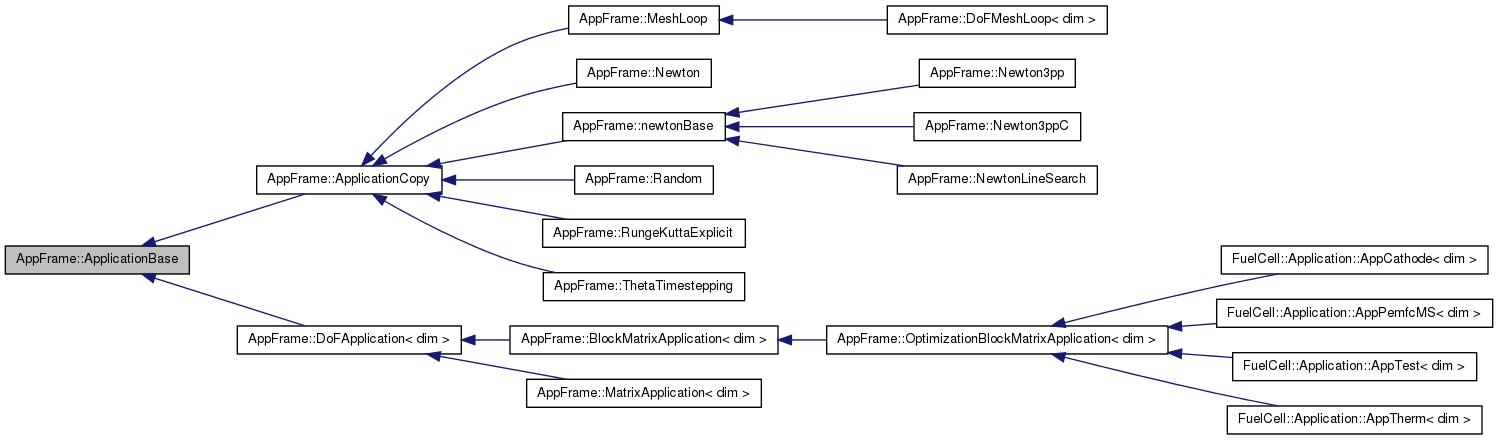
\includegraphics[width=\textwidth]{./figures/classAppFrame_ApplicationBase__inherit__graph.jpg}
\caption{Inheritance tree for ApplicationBase}
\label{fig:AppBase_Tree}
\end{center}
\end{figure}

Classes inherited from \textit{AppFrame::DoFApplication} are used when we need to implement the governing equations of the physical problem, i.e. the weak from of the partial differential equations. Class \textit{AppFrame::DoFApplication} implements all the methods used to assemble the right hand side, i.e. it contains a Triangularization (domain mesh), a deal.ii DoFHandler and several other objects to loop over cells. Class \textit{AppFrame:: BlockMatrixApplication} is a child of \textit{AppFrame::DoFApplication} and contains additional functionality in order to assemble and store the global system matrix into a BlockMatrix object. Finally, class \textit{AppFrame:: OptimizationBlockMatrixApplication} implements optimization functionality such as functional evaluation. OpenFCST applications that require assemble of a system matrix and right hand side are inherited from this application such as \textit{FuelCell::AppCathode}. 

Figure \ref{fig:AppCathode_Tree} provides an example of the inheritance tree for \textit{FuelCell::AppCathode}. AppCathode inherits all the functionality of of \textit{AppFrame::DoFApplication}, \textit{AppFrame::BlockMatrixApplication} and \textit{AppFrame:: OptimizationBlockMatrixApplication}. The responsibility of the OpenFCST applications in namespace \textit{FuelCell} is to initialize all the variables and to implement three main routines
\begin{itemize}
 \item cell\_matrix()
 \item cell\_residual()
 \item solve()
\end{itemize}
The first two routines are used to implement the element-wise system matrix and the element-wise right hand side. The latter member function is use to solve the global finite element problem. A tutorial on how to develop an application can be found in the HTML documentation.

Classes inherited from \textit{AppFrame::ApplicationCopy} are used to implement iterative loops. For example, when solving a nonlinear problem, a linear problem is solved iteratively. Therefore, classes that inherit from \textit{AppFrame::ApplicationCopy} usually contain an application that inherits from \textit{AppFrame::DoFApplication}. In terms of OpenFCST, OpenFCST developer will usually implement \textit{AppFrame::DoFApplication} and use the already implemented classes of type \textit{AppFrame::ApplicationCopy} in order to develop iterative loops for adaptive refinement, nonlinear problems and time-dependent problems.

As an example, in simulation\_builder.cc the following process is employed to solve a nonlinear problem:
\begin{lstlisting}
	//-- Select the application you want to run:
	app_lin = sim_selector->select_application();
	//-- Select the solver you want to run:
	newton = sim_selector->select_solver(app_lin.get());
	//-- Select the solving method you want to run, e.g. adaptive refinement:
	solver = sim_selector->select_solver_method(app_lin.get(), newton.get());
	// Here we have collected all information:
	deallog << "Run program using input file: " 
		<< simulator_parameter_file_name << std::endl;
	deallog.pop();
	solver->solve(simulator_parameter_file_name, param);
\end{lstlisting}
In the code above, first an OpenFCST application that inherits from \textit{AppFrame::DoFApplication} is created. Then, the application that is used to solve the linear system of governing equations at each iteration is handed in to a Newton solver that inherits from \textit{AppFrame::ApplicationCopy}. This solver is in turn handed to another solver that inherits from \textit{AppFrame::ApplicationCopy} and that implements an adaptive refinement loop.

Namespace \textit{FuelCell} is therefore a place holder for applications of type \textit{AppFrame::DoFApplication}. This applications are the core of OpenFCST since the assemble the system of equations that need to be solved. Users can develop their own applications by inheriting \textit{AppFrame::OptimizationBlockMatrixApplication} and re-implementing declare\_parameters(), initialize(), cell\_residual(), cell\_matrix() and solve() as shown in Figure \ref{fig:AppCathode_Tree} and explained in detail in the tutorial program for AppCathode. If the problem requires solving the problem iteratively such as in nonlinear and transient problems, the application will be handed over to an application of type \textit{AppFrame::ApplicationCopy} to be solved iteratively.

\begin{figure}[btp]
\begin{center} 
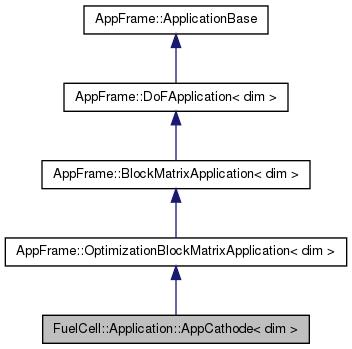
\includegraphics[scale=0.75]{./figures/classFuelCell_Application_AppCathode__inherit__graph.jpg}
\caption{Inheritance tree for FuelCell::Application::AppCathode}
\label{fig:AppCathode_Tree}
\end{center}
\end{figure}


The namespace \textit{FuelCellShop} is divided into several other namespaces as follows
\begin{enumerate}
 \item Material namespace: Specify the properties of common materials used in fuel cells. Examples of material classes include $PureGas$ baseclass.
 \item Layer namespace: Specify the different MEA components in a fuel cell. A BaseLayer has been developed in order to standarize this classes. They contain $material_id$ and $bondary_id$ elements to be able to relate the layer to the mesh as well as many other properties. Layer classes contain material classes in them that are used in order to obtain the appropriate physical parameters of the layer. Some layers are homogeneous and some are heterogeneous and anisotropic.
 \item Matrix namespace (OLD): Used to assemble the governing equations of a system. For linear problems this class implements the stiffness matrix for a givem equation. For nonlinear problems it generally includes $\frac{\partial R}{\partial \vec{u}}$. This matrix is used to calculate the step size in a Newton solver.
 \item Residual namespace (OLD): Used to assemble the governing equations of the system. For linear system these classes contain the right hand side of the problem. For nonlinear systems they contain the residual at the previous iteration, i.e. $R(\vec{u})$.
\end{enumerate}

%%===============================================================
\section{Layers Namespace}
%%===============================================================

A Layer in OpenFCST is used to define the properties of a cell in a finite element mesh. A Layer can be formed with with a single material or, in the case of composite layers such as a gas diffusion layer or a catalyst layer, it contains several materials and reaction parameters which are then used to compute the effective properties. An example of a catalyst layer is shown in Figure \ref{fig:catalystlayerexample}. 

\begin{figure}[tbp]
\begin{center}
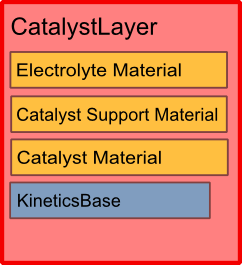
\includegraphics[width=0.25\textwidth]{figures/catalyst_layer_diagram.png}
\label{fig:catalystlayerexample}
\caption{Layer namespace structure}
\end{center}
\end{figure} 

The FuelCellShop::Layers namespace contains all the layers available with OpenFCST. All layers inherit from BaseLayer as shown in Figure \ref{fig:layerbase}. BaseLayer is a virutal class. An object of this class should never be created. BaseLayer simply provides common member functions and data members that apply to all layers. 



The layer classes contain a member function named set\_solution() which parses the uni

\begin{figure}
\begin{center}
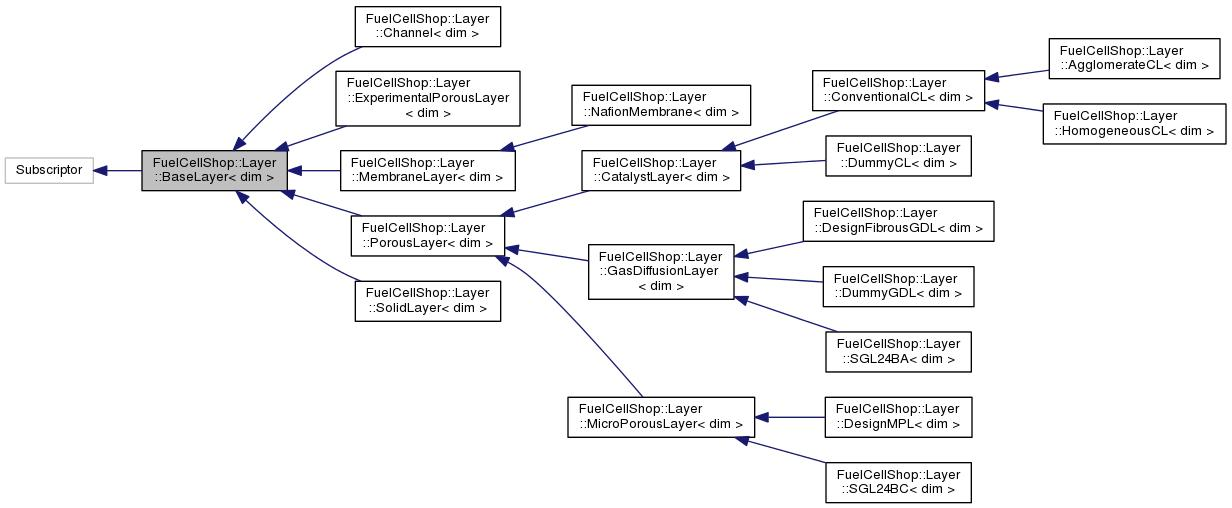
\includegraphics[width=0.9\textwidth]{figures/classFuelCellShop_1_1Layer_1_1BaseLayer__inherit__graph.jpg}
\label{fig:layerbase}
\caption{Layer namespace structure}
\end{center}
\end{figure} 





%%===============================================================
\section{Materials Namespace}
%%===============================================================

No materials contain a set solution. Materials will only set specific variables using a routine such as set\_temperature(double).






%%===============================================================
%%===============================================================
\section{Contributing libraries}

OpenFCST is distributed with copies of deal.II, Appframe, Dakota, COLDAE, ALGLIB and cpptest. These projects reside in the subdirectory \texttt{contrib/}. Please note that these projects are copyrighted by others than the OpenFCST authors and are covered by different licenses. For details, consult their respective webpages. A copy of their respective license is provided with the code. Inside each contributing library folder you will also find a file called \texttt{README.txt}. This file contains a list of any modifications that the OpenFCST developers have made to the contributing libraries. Note that some OpenFCST authors also contribute to the additional libraries. For example, Valentin Zingan is also contributor of the deal.II libraries.

\subsection{\texttt{APPFRAME}}
AppFrame was originally developed by Dr. Guido Kanschat at Texas A \& M and it is not continued to be developed by the ESDLab group. AppFrame is a framework to develop a chain of applications. The idea of these application classes is the possibility to build a chain out of these in order to have several predefined nested solvers. For this, we distinguish applications roughly in two classes, both derived from ApplicationBase:
\begin{itemize}
 \item Terminal applications, which implement the real finite element code like computing residuals on mesh cells, assembling matrices and solving linear systems.
 \item Non-terminal applications derived from ApplicationCopy; these usually implement a new solve() function as an iterative solver around another application. They implement all functions of the ApplicationBase interface, either forwarding them to the next inner application by ApplicationCopy or by providing their own implementation.
\end{itemize}

Usually a class in a chain communicates values with its next outer class through function arguments. Nevertheless, at least the terminal application will require values from even outer applications in the chain in order to compute residuals and matrices correctly. For these, the mechanism of named data provided by ApplicationData was introduced. Each class can store auxiliary data under a unique name there for use in inner iterations.

\subsubsection{Class DoFApplication}
This class it the parent of all terminal applications. It is the base class for applications requiring a Triangulation and a handler for degrees of freedom.

The mesh as well as the dof handler may be created by this class, which is the default, or they may be provided by another object, in which case they must be specified in the constructor.

Note that in this class the received or created dof handler is associated to the finite element given by the argument "Element" on the parameter file. Therefore, this class in not responsible to generate the system of equations to be solved, only to initialize the dof handler "Element" can either be a single element of a FESystem. In the latter case, the nomenclature used in the paramter file is: set Element = FESystem[element1\_type(element1\_degree)\textasciicircum number\_of\_elements1-...-elementN\_type(elementN\_degree)\textasciicircum number\_of\_elementsN] Example: set Element = FESystem[FE\_DGQ(0)-FE\_Q(1)\textasciicircum 2]

\subsubsection{Class BlockMatrixApplication}
\textbf{Text needed here}


\subsection{\texttt{COLDAE} Interface}
The class \texttt{DAESolver}, declared in \texttt{DAE\_solver.h} and defined in \texttt{DAE\_solver.cc}, provides an interface to the \texttt{Fortran 77} boundary-value differential algebraic equations (DAEs) code \texttt{COLDAE}.  The code solves DAEs the consists of a system of mixed-order ODEs
\begin{equation*}
  u_{i}^{(m_{i})} =  f_{i} ( x; z(u(x)), y(x) ), \quad    i = 1, ... ,c,
\end{equation*}
and algebraic constraints 
\begin{equation*}
  0   =  f_{i}( x; z(u(x)), y(x) ), \quad   i = c+1,...,c+d,
\end{equation*}
for $a < x < b$.   The DAE is subject to a system of mixed-point boundary conditions
\begin{equation*}
  g_{j}  ( \zeta_{j}; z(u(\zeta_{j})) ) = 0, \quad   j = 1, ... ,m^{*},
\end{equation*}
where 
\begin{equation*}
  a \leq \zeta_{1} \leq \zeta_{2} \leq \dots \leq \zeta_{m^{*}} \leq b,
\end{equation*}
and 
\begin{equation*}
  m^{*} = \sum^{c}_{i=1} m_{i}.
\end{equation*}
The code \texttt{COLDAE} returns an exact solution
\begin{equation*}
  z(u(x)) = ( u_{1}^{(1)}(x), u_{1}^{(m_{1}-1)}(x), \dots, u_{c}^{(m_{c}-1)}(x),
\end{equation*}
where $u_{i}^{(m_{i})}$ is the $i$th derivative of $u_{i}$.

The \texttt{COLDAE} interface is demonstrated by solving the DAEs
\begin{align*}
  z''(x) &= y(x) + \sin \left ( \frac{1}{1+x} \right ) + \frac{2}{(1+x)^{3}}, \quad 0 < x < 1, \\
  0 &= y(x) + \sin (z(x)),
\end{align*}
subject to the boundary conditions 
\begin{align*}
  z(0) &= 1, \\
  z(1) &= \frac{1}{2}.
\end{align*}

The DAE along with the boundary conditions are defined by a series of functions.  

Beginning with the DAE:
\begin{lstlisting}
void fsub(double &x, double z[], double y[], double f[])
{
	f[0] = y[0] + sin(1.0/(1.0+x)) + 2.0/pow(1.0+x,3);
	f[1] = y[0] + sin(z[0]);
}
\end{lstlisting}
In the above function, the functions \texttt{pow} and \texttt{sin} are declared in \texttt{math.h}.  The Jacobian matrix of the DAE must also be defined: 
\begin{lstlisting}
void dfsub(double &x, double z[], double y[], double df[])
{
	// Declare an array of pointers for the two dimensional array
	// that will hold the Jacobian matrix . 
    	double** dfc;
	dfc = new double*[2];
	for (int i=0; i < 2; ++i)
	{
		dfc[i] = new double[3];
		
	}
	
	// Define the Jacobian matrix.
	dfc[0][0] = 0.0;
	dfc[0][1] = 0.0;
	dfc[0][2] = 1.0;
	dfc[1][0] = cos(z[0]);
	dfc[1][1] = 0.0;
	dfc[1][2] = 1.0;
	
	// Convert the matrix dfc to a one dimensional
	// array that Fortran will understand. 
    	AppFrame::c_to_for_matrix(2,3,dfc,df);
}
\end{lstlisting}  
In the function \texttt{dfsub}, the function \texttt{AppFrame::c\_to\_for\_matrix} converts the \texttt{C/C++} two-dimensional array \texttt{dfc} to a one-dimensional array \texttt{df}.  The array \texttt{df} is then sent to \texttt{Fortran} and read as a two-dimensional array. Similar to the other math functions, \texttt{cos} is declared in \texttt{math.h}.  

The boundary conditions can be defined as:
\begin{lstlisting}
void gsub (int &i, double z[], double &g)
{	
	if (i == 1) g = z[0] - 1.0;
	else if (i == 2) g = z[0] - 1.0/2.0;  
}
\end{lstlisting}
In the above function, \texttt{i} refers to the location, between $ 0 \leq x \leq 1$, of the $i$th boundary condition.  In this case, \texttt{i==1} refers to $x=0$ and \texttt{i==2} refers to $x=1$. Similar to \texttt{fsub}, the partial derivatives must be defined for \texttt{gsub} in a separate function. 
\begin{lstlisting}
void dgsub (int &i, double z[], double dg[])
{
	if (i==1 || i == 2 )
	{
		dg[0] = 1.0;
		dg[1] = 0.0;
	}
		
}
\end{lstlisting}

Once the functions are defined, a few  variables must be defined that contains additional information about the boundary-value DAE.
\begin{lstlisting}
	//Declare an array that holds the 
	// order of each of the ODEs.
	int *mm = new int[1];
	mm[0] = 2;

	//Declare the location of each boundary point.
	double *zeta = new double[2];
	zeta[0] = 0.0;
	zeta[1] = 1.0;
\end{lstlisting} 

An instance of \texttt{DAESolver} can now be created by calling the constructor.
\begin{lstlisting}
	//Create an instance of the DAE solver class.  
	AppFrame::DAESolver *prob = new AppFrame::DAESolver
	(1,  //Number of ODES
	1, // Number of algebraic constraints
	mm, // Array that holds the order of each of the ODEs
	0.0, // Leftmost boundary point
	1.0, // Rightmost boundary point
	zeta, // Location of boundary points
	fsub, // ptr to ODE function
	dfsub, //ptr to Jacobian of ODE function
	gsub, //ptr to boundary-condition function
	dgsub, //ptr to derivatives of boundary-condition function
	);
\end{lstlisting}

Optional \texttt{COLDAE} parameters can be set by calling corresponding member function of the \texttt{DAESolver} class.  For example, the number of points in the initial mesh can be set.
\begin{lstlisting}
	prob->set_initial_mesh_size(20);
\end{lstlisting}
These methods must be called before the boundary-value DAE is solved.  See the \texttt{Doxygen} documentation for \texttt{DAESolver} for a complete list of methods.

Once all desired \texttt{COLDAE} parameters are set, the boundary-value DAE can be solved.
\begin{lstlisting}
	int flag = prob->DAE_solve();
\end{lstlisting}
The variable \texttt{flag} contains an integer value that reports the success of \texttt{COLDAE}; see \texttt{Doxygen} documentation.  If \texttt{COLDAE} is successful, a continuous solution can be accessed by the use of the \texttt{DAE\_solution} method.  For example, suppose a solution is required for $x=0.5$:
\begin{lstlisting}
	double x = 0.5; 
	double z[2];
	double y[1];
	prob->DAE_solution(x,z,y);
\end{lstlisting} 
In the above code, \texttt{z} contains the solution for the ODEs and \texttt{y} contains the solution for the algebraic constraints. 

%%===============================================================
%%===============================================================